% !TeX spellcheck = en_GB
%%=============================================================================
%% Toekomstvisie
%%=============================================================================
\chapter{\IfLanguageName{dutch}{Toekomstvisie}{Future vision}}
\label{ch:toekomstvisie}
This final chapter will focus on the public, private and on-premise solutions that Microsoft offers. 
Especially, how these are used as an extension of each other to build a modern infrastructure. 
It is not the first time that Microsoft Azure has been mentioned in this bachelor's thesis. 
It has been extensively used for the deployment of different proof of concept environments, as well as being mentioned in Chapter \ref{ch:stand-van-zaken}. 
The future of this environment will be discussed first. 
Afterwards, the future of their private cloud solution, Microsoft Azure Stack, will be examined. 
Furthermore, what can be expected from their on-premise solution, Windows Server 2019, in the future will be discussed. 
In particular the \acrlong{wac}, will be reviewed. 
The discussion of the different aspects exclusively has the intention to give the reader an idea of what the future can hold. 
It will be done cursory because all the different sections in this chapter contain sufficient content for their own bachelor's thesis. 
Finally, how these can be used in unison to form the infrastructure of tomorrow, as described in Figure \ref{fig:Azure_FullCircle}, will be concluded.

\begin{figure}[h]
	\captionsetup{width=0.6\linewidth}
	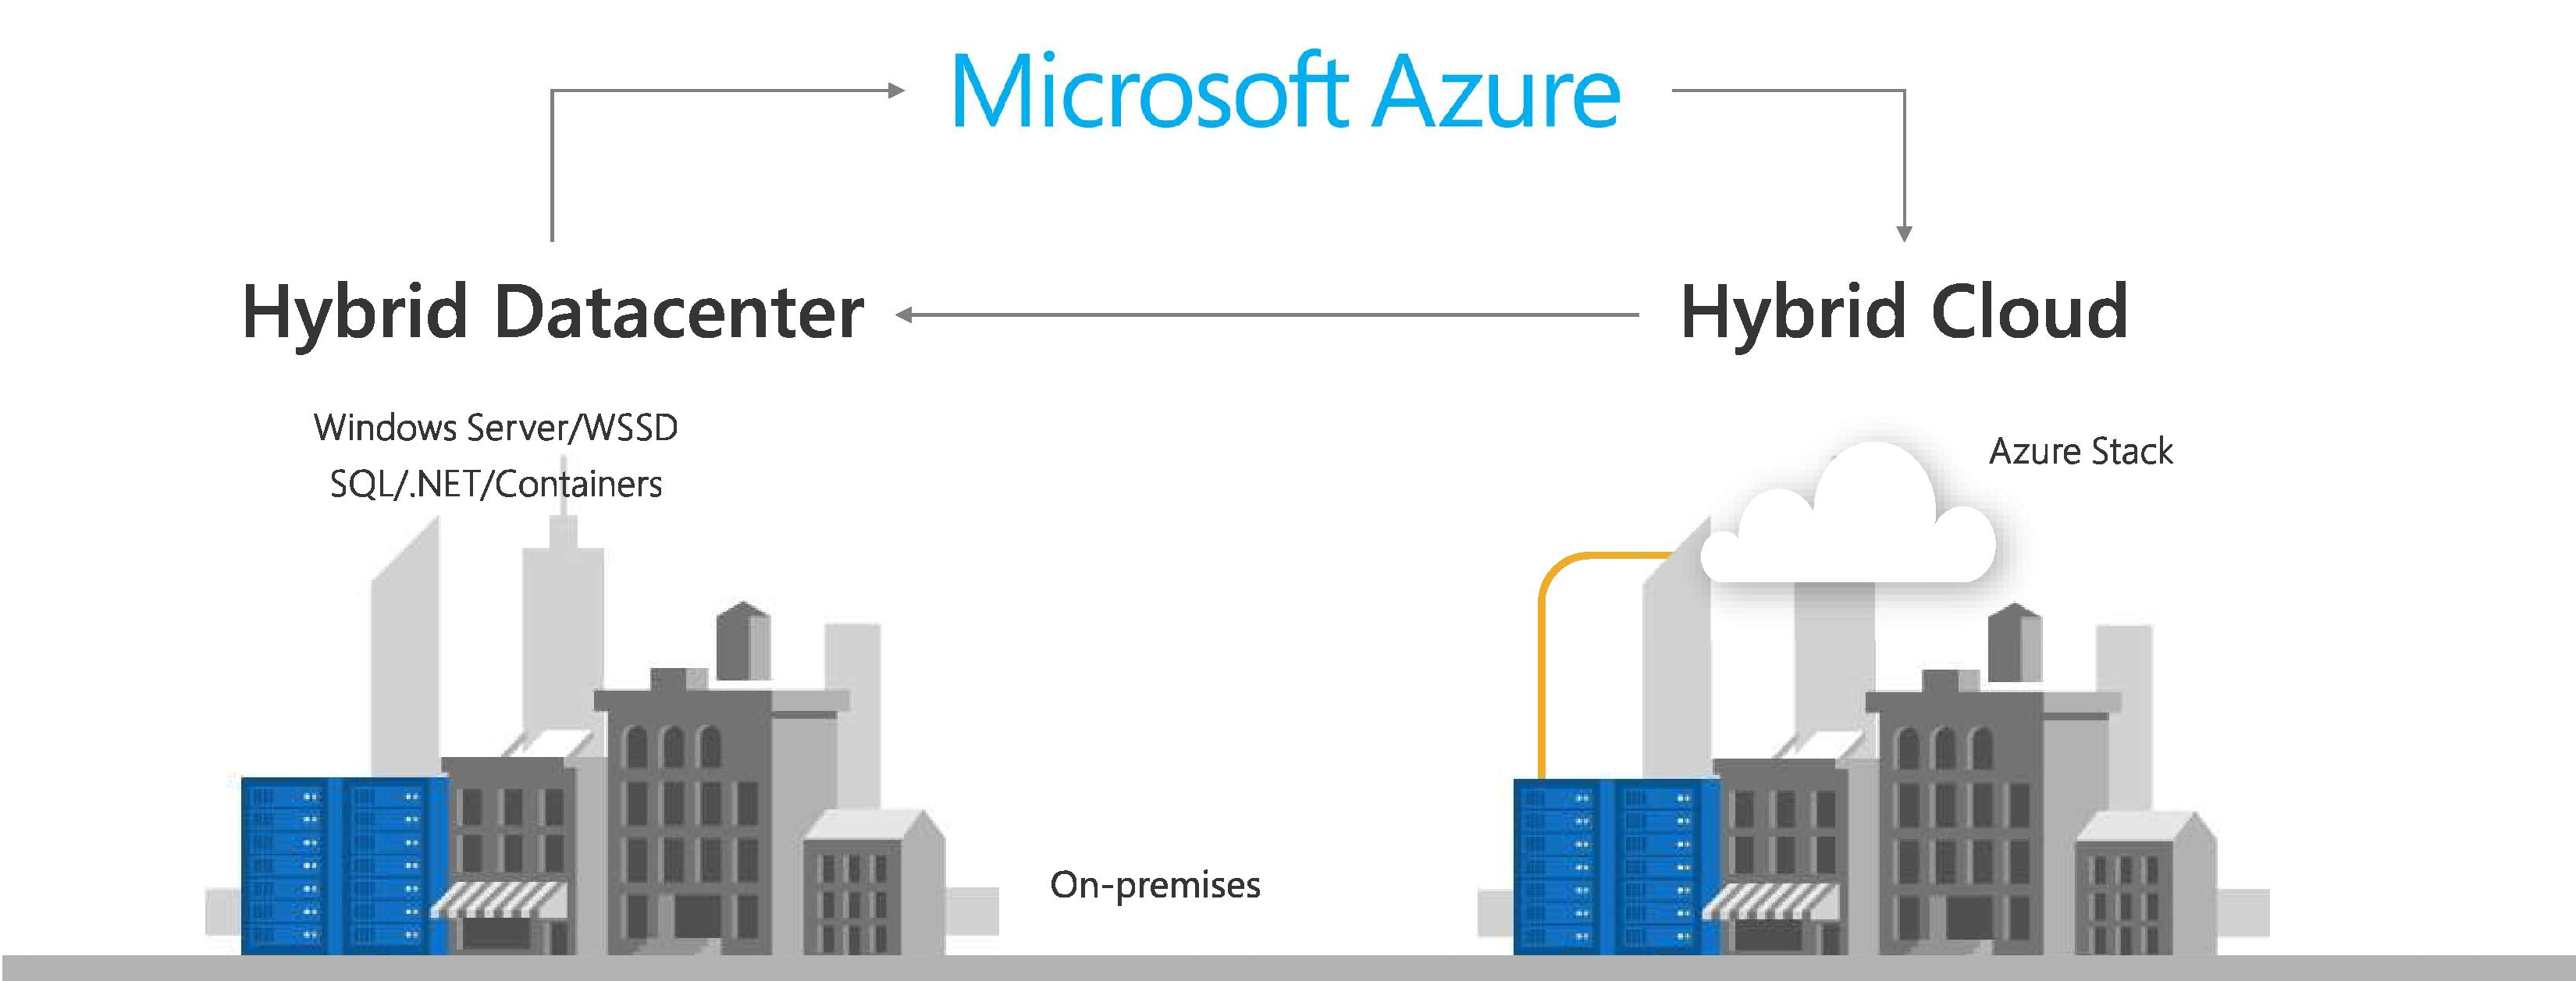
\includegraphics[width=0.7\linewidth]{img/Toekomstvisie/Azure1.png}
	\centering
	\caption[Modern infrastructure]{Bridging on-premise and cloud solutions for a modern infrastructure}
	\scriptsize	
	Adapted from \cite{Singh2019}
	\label{fig:Azure_FullCircle}
\end{figure}

\clearpage

\section{Microsoft Azure}
As previously mentioned, Microsoft Azure, is the public cloud solution Microsoft offers. 
There are currently more than fifty different global Azure regions and their network keeps expanding. 
It offers a wide array of solutions, some of which, like SAP on Azure, have been used in this bachelor's thesis. 
These are continuously updated to be on-par with the latest developments in \acrshort{it} such as \acrfull{ai} and blockchain. 
Microsoft also offers a selection of these services in China. 
These services can be managed from the Windows, macOS  and Linux \acrshort{os} through Azure Powershell. 
Alternatively they can be managed through the Azure Portal as can be seen in Figure \ref{fig:Azure_Portal}.

\begin{figure}[h]
	\captionsetup{width=0.8\linewidth}
	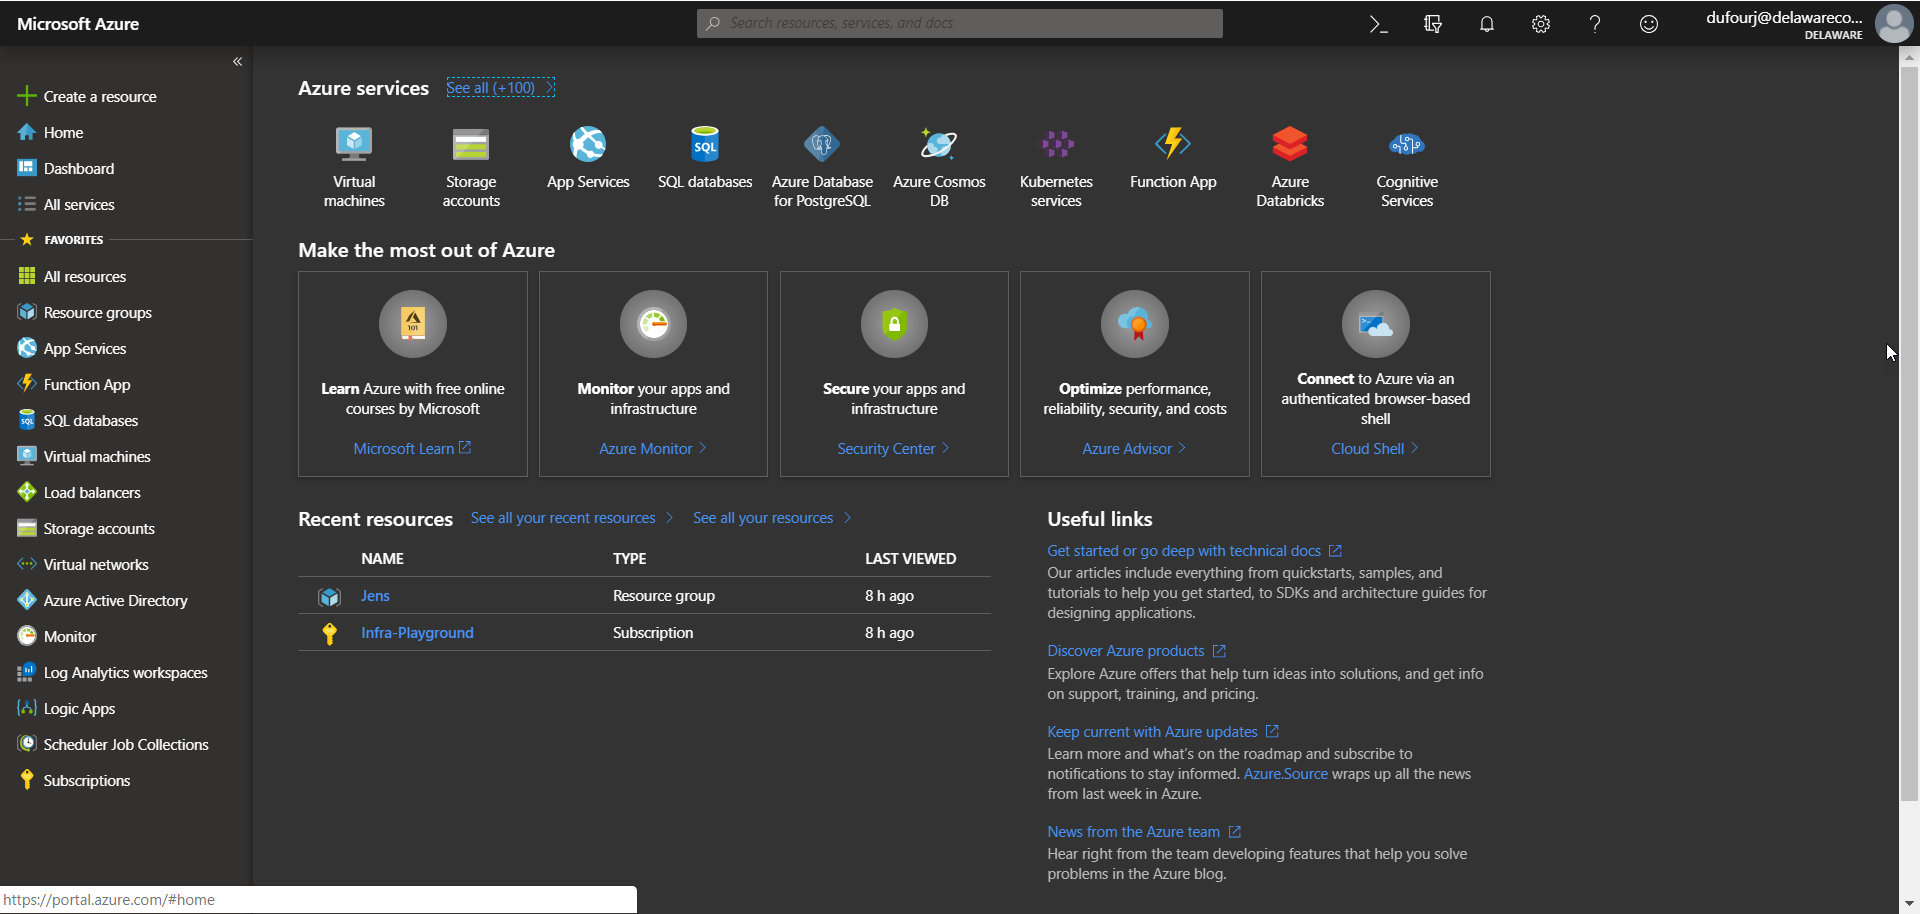
\includegraphics[width=0.9\linewidth]{img/Toekomstvisie/Azure0.png}
	\centering
	\caption[Azure Portal]{Microsoft Azure Portal landing page}
	\label{fig:Azure_Portal}
\end{figure}
Considering that the public cloud revenue is expected to grow 17.3\% in 2019, this is certainly one of the technologies that will play an important role in the future.\autocite{Ng2018}

\section{Microsoft Azure Stack}
As has been mentioned in Chapter \ref{ch:stand-van-zaken}, security concerns are one of the major bottlenecks when choosing for a public cloud. 
While most modern applications are being moved into the public cloud, some of these have additional requirements that can only be met by the usage of an on-premise solution. 
As an alternative, many organizations chose the additional security of a private cloud, a service that Microsoft offers through Microsoft Azure Stack. 
It allows organizations to run these applications in an on-premise environment, it brings the innovation of cloud computing to an on-premise environment.
It can be seamlessly integrated into Microsoft Azure to provide a hybrid cloud environment, which is an essential part of this bachelor's thesis, and of which the advantages have already been thoroughly discussed.

\section{\acrfull{wac}}
The final part of the puzzle that is going to be discussed is the \acrlong{wac}. 
It is an essential part of Windows Server 2019 and provides the resources to manage your on-premise infrastructure with the ease and efficiency that comes with a cloud solution. 
It also provides everything needed to interlink your public cloud, hosted on Microsoft Azure, with the on-premise infrastructure. 
Some features available, like Azure Site Recovery and Azure Backup, have already been discussed in Chapter \ref{ch:stand-van-zaken}, but it is important to note that a lot of new features are going to be added to the \acrlong{wac} over the following months.\autocite{Singh2019} 
\\
Features like Azure File Sync, file shares in the Azure public cloud, and Azure Migration, which will make the migration from Windows Server to Microsoft Azure even more fluent, have already been announced. 
\acrlong{wac} also, provides support for manufacturers extensions through its own \acrfull{sdk}. 	

\section{Conclusion}
As has been described in Figure \ref{fig:Azure_FullCircle}, Microsoft aims for a migration to the cloud. 
They want to provide an environment that distributes workloads dynamically, either between on-premise or cloud solutions. 
Windows Server 2019 was designed with this in mind, this is also explains why hybrid cloud and \acrshort{hci} are key themes in the \acrshort{os}. 
It is an \acrshort{os} that forms a bridge between the on-premise and cloud environments. 
It does this through the implementation of features, like \acrfull{s2d} and \acrfull{sdn}, which were previously only used in cloud environments. 
Microsoft aims to introduce new features several times a year that follow this ideology.
\\
They want to offer support to all of these components with a modern and future proof infrastructure in mind. 
Either by using a hybrid data centre, Windows Server 2019 combined with Microsoft Azure, or a hybrid cloud, Microsoft Azure combined with Microsoft Azure Stack.